% 库仑波函数
% 库仑函数|薛定谔方程|散射态|氢原子

\pentry{散射}% 链接未完成

本词条使用原子单位. 参考资料一个是 Wikipedia, 另一个是 “F Morales et al 2016 J. Phys. B: At. Mol. Opt. Phys. 49 245001” 的附录. 据说 Merzbacher 的量子力学也有.

\textbf{库仑波函数(Coulomb wave function)}是类氢原子% 链接未完成
的散射态波函数. % 链接未完成
库仑波函数常用的边界条件有两种, 以波数 $\bvec k$ 的平面波入射(球面波出射)的库仑波函数记为 $\psi_{\bvec k}^{(+)}(\bvec r)$, 平面波出射(球面波入射)的散射态记为 $\psi_{\bvec k}^{(-)}(\bvec r)$. 两种边界条件分别为
\begin{equation}
\psi_{\bvec k}^{(\pm)}(\bvec r) \to \frac{1}{(2\pi)^{3/2}} \E^{\I\bvec k\vdot\bvec r + \eta\ln (kr - \bvec k \vdot\bvec r)}
\qquad
(\bvec r\vdot \bvec k \to \mp\infty)
\end{equation}
库仑波函数的解析式为
\begin{equation}
\psi_{\bvec k}^{(\pm)}(\bvec r) = \frac{1}{(2\pi)^{3/2}} \Gamma(1\pm \I\eta)\E^{-\pi\eta/2} \E^{\I\bvec k\vdot\bvec r} {_1F_1}(\mp\I\eta; 1; \pm\I kr - \I \bvec k\vdot \bvec r)
\end{equation}
其中 $\eta = Z/k$, $\rho = kr$, $k$ 是能量为 $E = k^2/2$ 的平面波的波数, $Z$ 是原子核和电子的电荷之积(特别注意 $Z < 0$). 上式满足
\begin{equation}
\psi_{\bvec k}^{(+)}(\bvec r) = \psi_{-\bvec k}^{(-)}(r)^*
\end{equation}
\begin{equation}
\braket*{\psi_{\bvec k}^{(\pm)}}{\psi_{\bvec k'}^{(\pm)}} = \delta(\bvec k - \bvec k')
\end{equation}

\begin{figure}[ht]
\centering
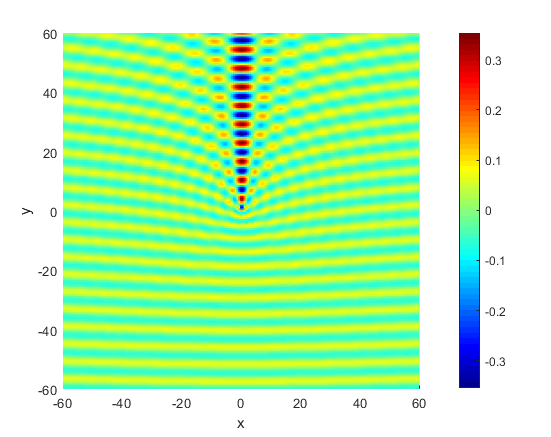
\includegraphics[width=12cm]{./figures/CulmWf_1.png}
\caption{$\psi_{\bvec k}^{(+)}(\bvec r)$ 的实部, $Z = -5$, $\bvec k = \bvec y$, $\eta = -5$. 当 $y \to -\infty$ 时趋近于平面波. 从经典力学考虑, 粒子越靠近原子核入射偏折越多. 注意左右两边的平面波偏折后会相交并产生干涉.} \label{CulmWf_fig2}
\end{figure}

\subsection{球坐标中的库仑波函数}
\pentry{薛定谔径向方程\upref{RadSE}}
球坐标中的库仑波函数与上面 “库仑平面波” 之间的关系, 可以类比平面波与球面波的关系\upref{Pl2Ylm}. 即 $k$ 相同的所有方向的平面波基底张成的空间与球面波基底张成的空间相同, 即能量为 $E = k^2/2$ 的无穷维子空间.

库仑势的薛定谔径向方程(\autoref{RadSE_eq1}\upref{RadSE})为
\begin{equation}
-\frac12 \dv[2]{u}{r} + \qty[\frac{Z}{r} + \frac{l(l+1)}{2 r^2}]u = \frac{k^2}{2}u
\end{equation}
其中 $u(r)$ 是 Scaled 波函数, $l$ 是角量子数. 方括号中的等效势能如\autoref{CulmWf_fig1}.
\begin{figure}[ht]
\centering
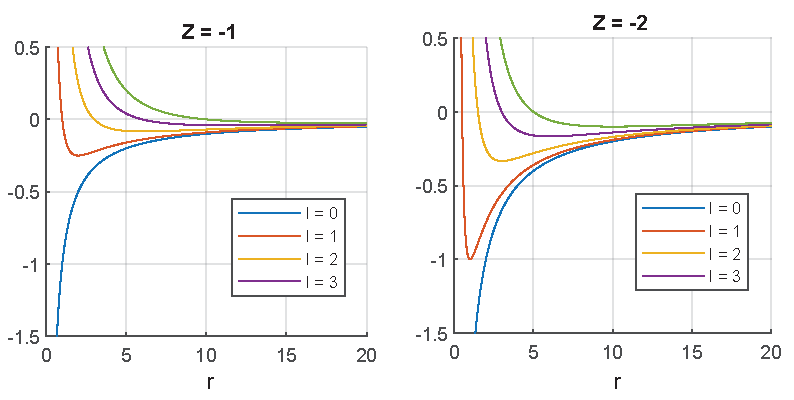
\includegraphics[width=12cm]{./figures/CulmWf_1.pdf}
\caption{球坐标中的径向等效势能} \label{CulmWf_fig1}
\end{figure}

将 $k, Z, r$ 换元为 $\eta, \rho$, 得
\begin{equation}
\dv[2]{u}{\rho} + \qty[1 - \frac{2\eta}{\rho} - \frac{l(l+1)}{\rho^2}]u = 0
\end{equation}
两个线性无关解为\textbf{第一类库仑函数} $F_l(\eta, \rho)$ 和\textbf{第二类库仑函数} $G_l(\eta, \rho)$\upref{CulmF}. 散射态中, 我们假设 $k > 0$ ($E > 0$). 但理论上我们也可以取 $k$ 为正虚数 ($E < 0$), 这样当 $E$ 为束缚态能量时就可以得到束缚态的波函数(见\autoref{HWF_eq2}\upref{HWF}).

所以完备正交归一的\textbf{库仑球面波}为
\begin{equation}\label{CulmWf_eq1}
\ket{C_{l,m}(k)} = \frac{1}{r} \sqrt{\frac{2}{\pi}} F_l(\eta, kr) Y_{l,m}(\uvec r)
\end{equation}
满足
\begin{equation}\label{CulmWf_eq2}
\braket{C_{l',m'}(k')}{C_{l,m}(k)} = \delta_{l,l'}\delta_{m,m'}\delta(k-k')
\end{equation}

现在可以将库仑波函数展开为
\begin{equation}\label{CulmWf_eq9}
\psi_{\bvec k}^{(\pm)}(\bvec r) =  \sum_{l,m} a_{l,m}^{(\pm)}(\bvec k) \ket{C_{l,m}(k)}
\end{equation}
其中
\begin{equation}% (-) 有待验证
a_{l,m}^{(\pm)}(\bvec k) = \frac{\I^l}{k} \exp[\pm\I\sigma_l(Z/k)] Y_{l,m}^* (\uvec k)
\end{equation}
$\sigma$ 是库仑相移(\autoref{CulmF_eq8}\upref{CulmF}). 注意 $a_{l,m}$ 并不是 $\braket*{C_{l,m}(k)}{\psi_{\bvec k}^{(\pm)}}$, 后者模长为无穷大, 也可记为 $a_{l,m}\delta(0)$.

与平面波的情况(傅里叶变换)类似, 要将一个球谐展开的波函数 $\ket{f}$ 投影到库仑波函数上, 就先投影到库仑球面波上, 然后进行幺正变换
\begin{equation}
\braket*{\psi_{\bvec k}^{(\pm)}}{f} = \sum_{l,m}  a_{l,m}^{(\pm)}(\bvec k)^* \braket{C_{l,m}(k)}{f}
\end{equation}
若 $\ket{f}$ 的 scaled 径向波函数为 $u_{l,m}(r)$, 则
\begin{equation}
\braket*{\psi_{\bvec k}^{(\pm)}}{f} = \frac{1}{k} \sum_{l,m} g_{l,m}(k) Y_{l,m}(\uvec k)
\end{equation}
其中
\begin{equation}
g_{l,m}(k) = \sqrt{\frac{2}{\pi}} \I^{-l} \E^{\mp\I\sigma_l} \int_0^\infty F_l(\eta, kr) u_{l,m}(r) \dd{r}
\end{equation}

将波函数做傅里叶变换和投影到库仑波函数有什么区别呢? 例如做氢原子电离的 TDSE, 若想求 $t = +\infty$ 时的动量分布, 理论上只要在 $t$ 足够大时做傅里叶变换即可, 但如果 $t$ 不够大(电场已消失), 电离波包所受的库仑力还不可忽略, 那么虽然得到了瞬时的动量分布, 但却与 $t = +\infty$ 的不同. 这时因为动量算符与哈密顿算符不对易, 动量不守恒. 但若在电场消失的时候, 投影到 $\psi_{\bvec k}^{(-)}$ 上, 由于它是哈密顿的本征函数, 投影的模方(概率)不会随时间改变.

最后的问题就是, 当 $t = +\infty$ 时, 投影到平面波和库仑波是否相同呢? 要验证这一点, 只需验证
\begin{equation}
\braket*{\psi_{\bvec k}^{(-)}}{\bvec k'} = \delta(\bvec k - \bvec k')
\end{equation}
我们还是用球谐展开来验证
\begin{equation}\ali{
\braket*{\psi_{\bvec k}^{(\pm)}}{\bvec k'} &= \sum_{l,m} \braket*{\psi_{\bvec k}^{(\pm)}}{C_{l,m}(k)}\ket{C_{l,m}(k)} \sum_{l',m'} \bra{s_{l',m'}(k')}\braket{s_{l',m'}(k')}{\bvec k'} \\
&= \sum_{l,m} \braket*{\psi_{\bvec k}^{(\pm)}}{C_{l,m}(k)}\braket{C_{l,m}(k)}{s_{l,m}(k')}\braket{s_{l,m}(k')}{\bvec k'}
}\end{equation}
(但是径向积分貌似不会做, 就当是对的吧).
